

\tikzset{every picture/.style={line width=0.75pt}} %set default line width to 0.75pt        

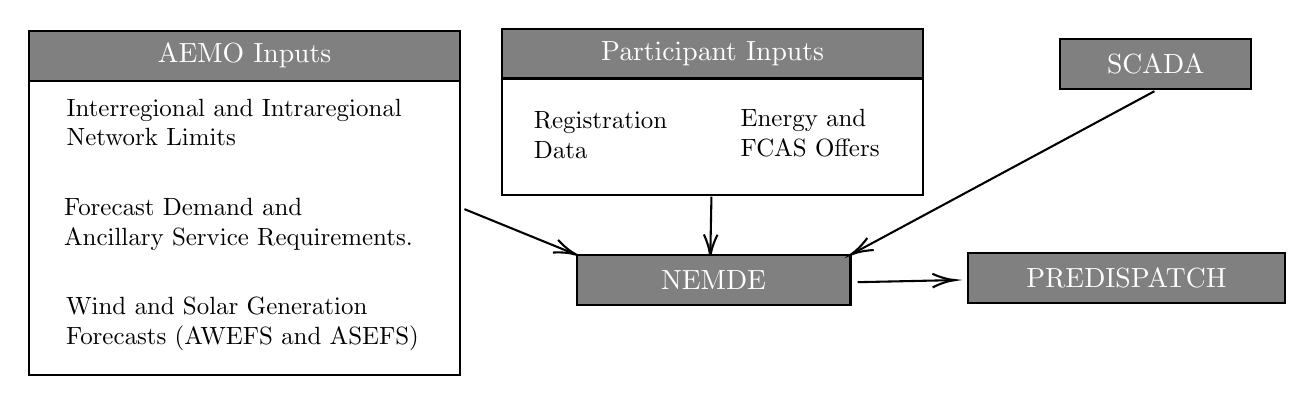
\begin{tikzpicture}[x=0.75pt,y=0.75pt,yscale=-1,xscale=1]
%uncomment if require: \path (0,191.0132598876953); %set diagram left start at 0, and has height of 191.0132598876953

%Straight Lines [id:da9177958313522097] 
\draw    (357.44,91.83) -- (356.91,119.02) ;
\draw [shift={(356.87,121.02)}, rotate = 271.13] [color={rgb, 255:red, 0; green, 0; blue, 0 }  ][line width=0.75]    (10.93,-3.29) .. controls (6.95,-1.4) and (3.31,-0.3) .. (0,0) .. controls (3.31,0.3) and (6.95,1.4) .. (10.93,3.29)   ;

%Straight Lines [id:da12798518797085823] 
\draw    (238.44,97.83) -- (290.59,119.07) ;
\draw [shift={(292.44,119.83)}, rotate = 202.17000000000002] [color={rgb, 255:red, 0; green, 0; blue, 0 }  ][line width=0.75]    (10.93,-3.29) .. controls (6.95,-1.4) and (3.31,-0.3) .. (0,0) .. controls (3.31,0.3) and (6.95,1.4) .. (10.93,3.29)   ;

%Shape: Rectangle [id:dp13477801690658042] 
\draw   (256.5,10.9) -- (459.5,10.9) -- (459.5,90.9) -- (256.5,90.9) -- cycle ;
%Shape: Rectangle [id:dp8582430372753662] 
\draw  [fill={rgb, 255:red, 128; green, 128; blue, 128 }  ,fill opacity=1 ] (256.5,10.9) -- (459.5,10.9) -- (459.5,34.9) -- (256.5,34.9) -- cycle ;
%Shape: Rectangle [id:dp5655505133083187] 
\draw   (28.5,11.9) -- (236.44,11.9) -- (236.44,177.9) -- (28.5,177.9) -- cycle ;
%Shape: Rectangle [id:dp5185219575052318] 
\draw  [fill={rgb, 255:red, 128; green, 128; blue, 128 }  ,fill opacity=1 ] (28.5,11.9) -- (236.44,11.9) -- (236.44,35.9) -- (28.5,35.9) -- cycle ;


%Shape: Rectangle [id:dp11057728244309994] 
\draw  [fill={rgb, 255:red, 128; green, 128; blue, 128 }  ,fill opacity=1 ] (292.44,119.83) -- (424.44,119.83) -- (424.44,143.83) -- (292.44,143.83) -- cycle ;
%Shape: Rectangle [id:dp07113446577922766] 
\draw  [fill={rgb, 255:red, 128; green, 128; blue, 128 }  ,fill opacity=1 ] (525.5,15.9) -- (617.44,15.9) -- (617.44,39.9) -- (525.5,39.9) -- cycle ;

%Straight Lines [id:da9707191163095252] 
\draw    (570.87,41.02) -- (426.2,118.88) ;
\draw [shift={(424.44,119.83)}, rotate = 331.71000000000004] [color={rgb, 255:red, 0; green, 0; blue, 0 }  ][line width=0.75]    (10.93,-3.29) .. controls (6.95,-1.4) and (3.31,-0.3) .. (0,0) .. controls (3.31,0.3) and (6.95,1.4) .. (10.93,3.29)   ;

%Shape: Rectangle [id:dp46501665361769806] 
\draw  [fill={rgb, 255:red, 128; green, 128; blue, 128 }  ,fill opacity=1 ] (480.87,118.83) -- (633.87,118.83) -- (633.87,142.83) -- (480.87,142.83) -- cycle ;
%Straight Lines [id:da4584246014213331] 
\draw    (427.87,133.02) -- (472.87,132.06) ;
\draw [shift={(474.87,132.02)}, rotate = 538.78] [color={rgb, 255:red, 0; green, 0; blue, 0 }  ][line width=0.75]    (10.93,-3.29) .. controls (6.95,-1.4) and (3.31,-0.3) .. (0,0) .. controls (3.31,0.3) and (6.95,1.4) .. (10.93,3.29)   ;


% Text Node
\draw (358,22.9) node [color={rgb, 255:red, 255; green, 255; blue, 255 }  ,opacity=1 ] [align=left] {Participant Inputs};
% Text Node
\draw (304,62) node [scale=0.9] [align=left] {Registration\\Data};
% Text Node
\draw (405,61) node [scale=0.9] [align=left] {Energy and\\FCAS Offers};
% Text Node
\draw (132.47,23.9) node [color={rgb, 255:red, 255; green, 255; blue, 255 }  ,opacity=1 ] [align=left] {AEMO Inputs};
% Text Node
\draw (129.53,105) node [scale=0.9] [align=left] {Forecast Demand and \\Ancillary Service Requirements.};
% Text Node
\draw (127.5,56) node [scale=0.9] [align=left] {Interregional and Intraregional \\Network Limits};
% Text Node
\draw (131.5,153) node [scale=0.9] [align=left] {Wind and Solar Generation \\Forecasts (AWEFS and ASEFS)};
% Text Node
\draw (571.47,27.9) node [color={rgb, 255:red, 255; green, 255; blue, 255 }  ,opacity=1 ] [align=left] {SCADA};
% Text Node
\draw (358.44,131.83) node [color={rgb, 255:red, 255; green, 255; blue, 255 }  ,opacity=1 ] [align=left] {NEMDE};
% Text Node
\draw (557.37,130.83) node [color={rgb, 255:red, 255; green, 255; blue, 255 }  ,opacity=1 ] [align=left] {PREDISPATCH};


\end{tikzpicture}
